\chapter{DATA TRANSMISSION}

\section{Program Input and Output}

Workpiece programs (main programs \textbf{PM} and subprograms \textbf{MM}) can be entered and output in all operating modes of the control, whether the machine is stopped or running.

The active program can also be output at any time.

Before entering or outputting programs, the peripheral equipment must be connected to the control system using the appropriate cable for data transmission.

The peripheral equipment must be ready for operation.

\subsection{Entering Programs from an External Data Storage}

When programs are entered, the control system verifies all data introduced by the external data storage for errors.

If an error (such as an invalid character, excessive length of a word or block, etc.) is detected, the control system automatically interrupts the input process, and an error message appears on the display screen.

A program that has been incompletely entered must be deleted from the memory of the main program or subprogram, as otherwise, it will not be possible to enter a program with the same number again.

For program deletion, see paragraph 6.5.1.

It is possible to enter not only all programs at once from an external data storage device but also individual programs.

\newpage

\subsubsection{Entering All Programs into Memory}

\textbf{Select the PM or MM memory}  
(Follow the procedure described in paragraph 6.5.1).

The list of program numbers stored in the main program memory or subprogram memory appears on the screen:

\begin{center}
    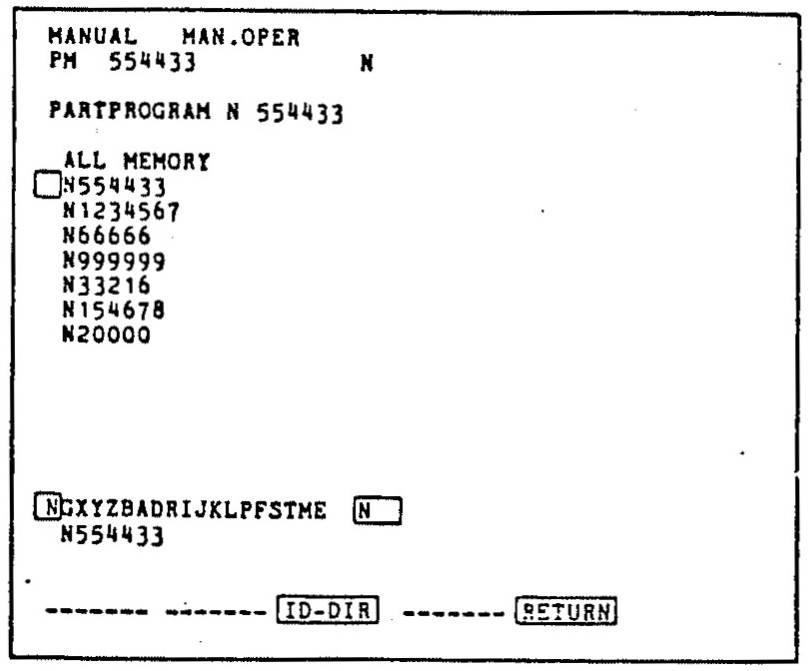
\includegraphics[width=0.6\linewidth]{program_list.jpg}
\end{center}

\begin{itemize}
    \iconitem{Move the cursor to the \textbf{ALL MEMORY} line by pressing the up/down command buttons.}{up.jpg, down.jpg}
\end{itemize}

\vspace{.5cm}

\begin{itemize}
    \iconitem{Press the \textbf{DATA IN/OUT} button.}{data_in_out.jpg}
\end{itemize}

\vspace{.5cm}

\begin{itemize}
    \iconitem{Press the function button \textbf{F1} (INPUT). (This introduces data from an external storage device.)}{f1.jpg}
\end{itemize}

The \textbf{IN} signal (indicating data entry from an external storage device) appears on line 5 of the screen.

Programs are entered into the control system one after another.

The \textbf{CODE}, \textbf{program number}, and \textbf{sequence number} of the entered program are displayed on line 5 of the screen:

\begin{center}
    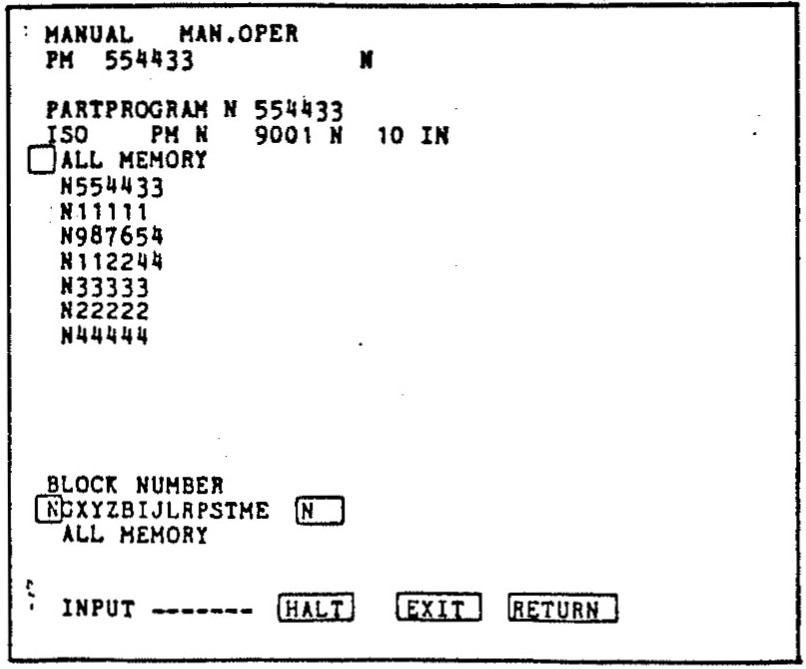
\includegraphics[width=0.6\linewidth]{program_entry.jpg}
\end{center}

\newpage

The program numbers entered are now listed at the end of the program number list.

\notes

The input procedure can be stopped at any time by pressing the function key \textbf{F3 (HALT)} and resumed by pressing the function key \textbf{F1 (INPUT)}.

Data entry can be terminated at any time using the function key \textbf{F4 (EXIT)}.

After stopping the procedure, the last entered program must be erased from the control system's memory; otherwise, a program with this number cannot be entered again.

\subsubsection{Introduction of a Single Program into Memory}

\textbf{Selecting Memory PM or MM}  
(Follow the procedure described in paragraph \textbf{6.5.1}.)

On the screen, the list of program numbers from the main program memory or the subprogram memory, previously stored with \textbf{PM} or \textbf{MM}, appears.

\begin{itemize}
    \item Enter the program number \textbf{N} on the numeric keypad.
    \iconitem{Press the \textbf{ENTER} key.}{enter.jpg}
\end{itemize}

\vspace{.5cm}

The program number \textbf{N} to be entered is displayed on line 21 of the screen.

\begin{itemize}
    \iconitem{Press the \textbf{DATA IN/OUT} key to start the input procedure.}{data_in_out.jpg}
\end{itemize}

\vspace{.5cm}

\begin{itemize}
    \iconitem{Press the function key \textbf{F1 (ONPUT)}.}{f1.jpg}
\end{itemize}

The \textbf{CODE}, the program number, and the sequence numbers are displayed on line 5 of the screen.

The program to be entered is retrieved from the external information support and then stored in the system control memory.

At the end of the input procedure, the cursor is returned to the first program number in the list of program numbers.

The program number of the entered program is now listed at the end of the program number list.

\notes

The input procedure can be stopped at any time by pressing the function key \textbf{F3 (HALT)} and resumed by pressing the function key \textbf{F1 (INPUT)}.

The input procedure can also be terminated at any time using the function key \textbf{F4 (EXIT)}.

After stopping the procedure, the last entered program must be erased from the control system's memory; otherwise, a program with this number cannot be entered again.

\newpage

\subsection{Output of Programs to an External Information Support}

It is possible to transfer not only all programs together but also each program individually from the control system to an external information support.

\subsubsection{Output of All Programs}

\textbf{Selecting Memory PM or MM}  
(Follow the procedure described in paragraph \textbf{6.5.1}.)

On the screen, the list of program numbers from the main program memory or the subprogram memory, previously stored with \textbf{PM} or \textbf{MM}, appears.

\begin{center}
    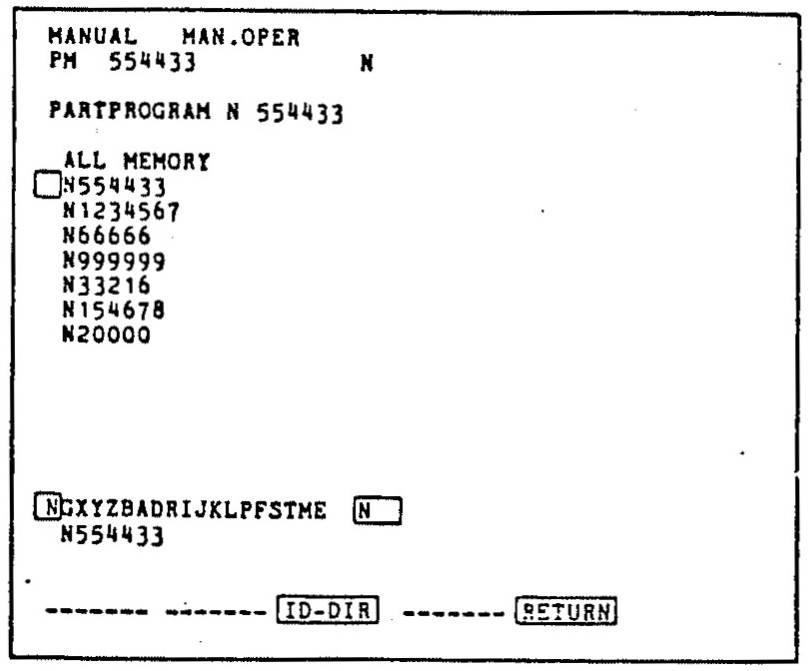
\includegraphics[width=0.6\linewidth]{program_list.jpg}
\end{center}

\begin{itemize}
    \iconitem{Move the cursor to the \textbf{ALL MEMORY} line using the up/down command keys.}{up.jpg, down.jpg}
\end{itemize}

\vspace{.5cm}

\begin{itemize}
    \iconitem{Press the \textbf{DATA IN/OUT} key.}{data_in_out.jpg}
\end{itemize}

\vspace{.5cm}

\begin{itemize}
    \iconitem{Press the function key \textbf{F2 (OUTPUT)}.}{f2.jpg}
\end{itemize}

The programs are transferred from the control system and read one after another.

The \textbf{CODE}, the program number being read, and the sequence numbers of this program are displayed on line 5 of the screen.

\notes

The reading procedure can be stopped at any time by pressing the function key \textbf{F3 (HALT)} and resumed by pressing the function key \textbf{F2 (OUTPUT)}.

The reading procedure can also be terminated at any time using the function key \textbf{F4 (EXIT)}.

\newpage

\subsubsection{Output of a Single Program}

\textbf{Selecting Memory PM or MM}  
(Follow the procedure described in paragraph \textbf{6.5.1}.)

On the screen, the list of program numbers from the main program memory or the subprogram memory, previously stored with \textbf{PM} or \textbf{MM}, appears.

\begin{itemize}
    \item Enter the program number \textbf{N} on the numeric keypad.
    \iconitem{Press the \textbf{ENTER} key.}{enter.jpg}
\end{itemize}

\vspace{.5cm}

The program number \textbf{N} to be read appears on line 21 of the screen.

\begin{itemize}
    \iconitem{Press the \textbf{DATA IN/OUT} key to start the readout procedure.}{data_in_out.jpg}
\end{itemize}

\vspace{.5cm}

\begin{itemize}
    \iconitem{Press the function key \textbf{F2 (OUTPUT)}.}{f2.jpg}
\end{itemize}

The program to be read is transferred from the control system.  
The \textbf{CODE}, the program number being read, and the sequence numbers of this program are displayed on line 5 of the screen.

\notes

The program number \textbf{N} to be read can also be searched by using the cursor command keys \textbf{"up-down"}.

The readout procedure can be stopped at any time by pressing the function key \textbf{F3 (HALT)} and resumed by pressing the function key \textbf{F2 (OUTPUT)}.

The readout procedure can also be terminated at any time using the function key \textbf{F4 (EXIT)}.

\section{Introduction and Readout of Specified Data}

The introduction and readout of the indicated data below can only be performed in \textbf{MANUAL} mode:

\begin{itemize}
    \item \underline{Tool data}
    \item \underline{Tool service life}
    \item \underline{Spare tools}
    \item \underline{Origin offsets}
    \item \underline{Parameters}
    \item \underline{Point definition}
\end{itemize}

The introduction or readout of numbers \textbf{P} for tool placement in the tool magazine (see paragraph \textbf{4.1.6}) is not possible.

The peripheral equipment must be connected to the control system using the appropriate data transmission cable before proceeding with data introduction or readout.  
The peripheral equipment must be in operating condition.

The memory introduction and readout procedures can be stopped or terminated at any time  
(see description under \textbf{8.1.1.2} and \textbf{8.1.2.2} "Remarks").

If an error is detected, the control system automatically interrupts the introduction procedure, and the error message is displayed on the screen.

After an interruption of the introduction procedure, any incomplete data must be verified and completed or erased and reintroduced into memory \textbf{TM, TL, TS}, or \textbf{ZO}, as applicable.

\newpage

\subsection{Introduction of Tool Data from an External Data Support}

\begin{itemize}
    \iconitem{Press the \textbf{MANUAL} key.}{manual.jpg}
\end{itemize}

\vspace{.5cm}

\begin{itemize}
    \iconitem{Press the \textbf{TOOL MEM} key.}{tool_mem.jpg}
\end{itemize}
\vspace{.5cm}
The tool data list appears on the screen:

\begin{center}
    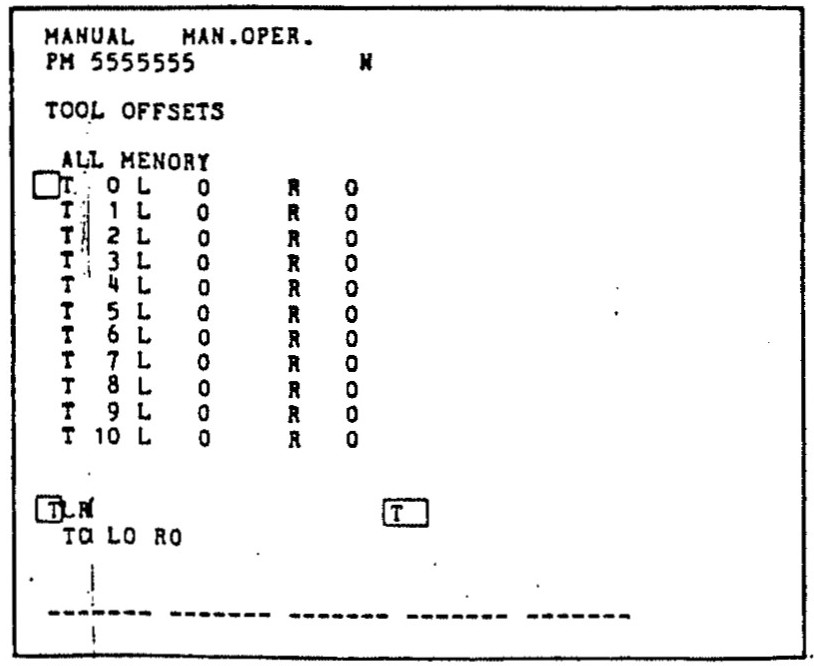
\includegraphics[width=0.6\linewidth]{tool_data_screen.jpg}
\end{center}

\begin{itemize}
    \iconitem{Press the \textbf{DATA IN/OUT} key.}{data_in_out.jpg}
\end{itemize}

\vspace{.5cm}

\begin{itemize}
    \iconitem{Press the function key \textbf{F1 (INPUT)}.}{f1.jpg}
\end{itemize}

The tool data is then stored in the system's tool data memory \textbf{TOOL OFFSETS}.

The tool numbers \textbf{I} are displayed on line 5 of the screen.

\newpage

\subsection{Output of Tool Data to an External Data Support}

It is possible to transfer all tool data from the system’s \textbf{TM} tool data memory to an external information support.

\subsubsection{Output of All Data}

\begin{itemize}
    \iconitem{Press the \textbf{MANUAL} key.}{manual.jpg}
\end{itemize}

\vspace{.5cm}

\begin{itemize}
    \iconitem{Press the \textbf{TOOL MEM} key.}{tool_mem.jpg}
\end{itemize}

The tool data list appears on the screen:

\begin{center}
    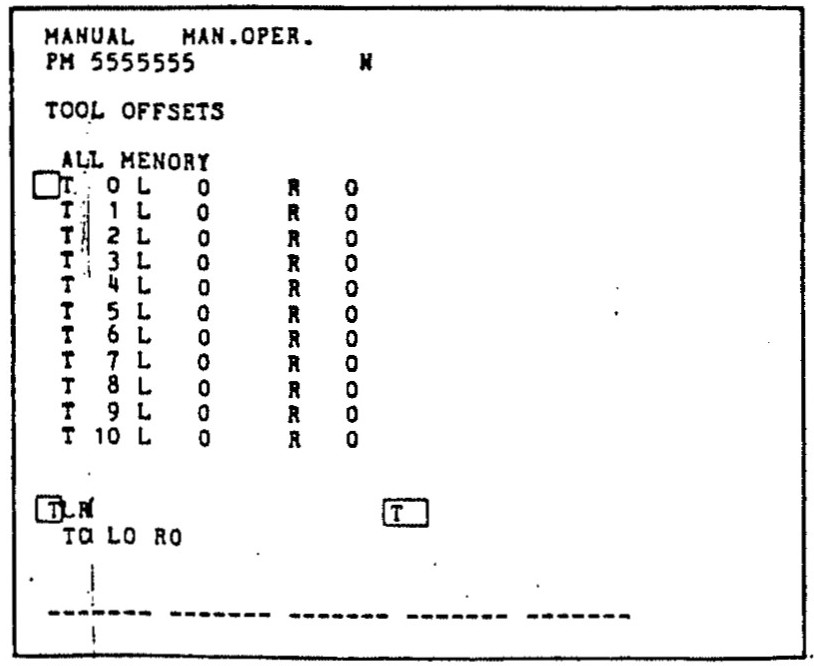
\includegraphics[width=0.6\linewidth]{tool_data_screen.jpg}
\end{center}

\begin{itemize}
    \iconitem{Move the cursor to the \textbf{ALL MEMORY} line using the up/down command keys.}{up.jpg, down.jpg}
\end{itemize}

\vspace{.5cm}

\begin{itemize}
    \iconitem{Press the \textbf{DATA IN/OUT} key.}{data_in_out.jpg}
\end{itemize}

\vspace{.5cm}

\begin{itemize}
    \iconitem{Press the function key \textbf{F2 (OUTPUT)}.}{f2.jpg}
\end{itemize}

The \textbf{OUT} signal (readout to an external information support) is displayed on line 5 of the screen.

The tool data is transferred from the system’s tool data memory \textbf{TOOL OFFSETS}.

The tool numbers \textbf{I} are displayed on line 5 of the screen.

\newpage

\subsection{Introduction and Readout of Tool Service Life Data}

\begin{itemize}
    \iconitem{Press the \textbf{MANUAL} key.}{manual.jpg}
\end{itemize}

\vspace{.5cm}

\begin{itemize}
    \iconitem{Press the \textbf{TOOL MEM} key.}{tool_mem.jpg}
\end{itemize}

\vspace{.5cm}

\begin{itemize}
    \iconitem{Press the \textbf{MENU} key.}{menu.jpg}
\end{itemize}

The submenu for tool programming appears on the screen.

\begin{itemize}
    \item Enter the number \textbf{1} on the numeric keypad to select \textbf{EDIT TOOL LIFE}.
    \item (Introduction and modification of tool service life data).
\end{itemize}

The list of tool service life data appears on the screen.

\begin{itemize}
    \iconitem{Press the \textbf{DATA IN/OUT} key.}{data_in_out.jpg}
\end{itemize}

\vspace{.5cm}

\begin{itemize}
    \iconitem{Press the function key \textbf{F1 (INPUT)} or \textbf{F2 (OUTPUT)}.}{f1.jpg, f2.jpg}
\end{itemize}

The \textbf{IN} signal (data input from an external information support) or the \textbf{OUT} signal (readout to an external information support) appears on line 5 of the screen.

The tool service life data is then either stored in the \textbf{TL} tool life memory of the system or transferred to an external support.

The tool numbers \textbf{T} are displayed on line 5 of the screen.

\subsection{Introduction and Readout of Spare Tools}

\begin{itemize}
    \iconitem{Press the \textbf{MANUAL} key.}{manual.jpg}
\end{itemize}

\vspace{.5cm}

\begin{itemize}
    \iconitem{Press the \textbf{TOOL MEM} key.}{tool_mem.jpg}
\end{itemize}

\vspace{.5cm}

\begin{itemize}
    \iconitem{Press the \textbf{MENU} key.}{menu.jpg}
\end{itemize}

The submenu for tool programming appears on the screen.

\begin{itemize}
    \item Enter the number \textbf{2} on the numeric keypad to select \textbf{EDIT TOOL SPARE}.
\end{itemize}

The list of spare tool numbers appears on the screen.

\begin{itemize}
    \iconitem{Press the \textbf{DATA IN/OUT} key.}{data_in_out.jpg}
\end{itemize}

\vspace{.5cm}

\begin{itemize}
    \iconitem{Press the function key \textbf{F1 (INPUT)} or \textbf{F2 (OUTPUT)}.}{f1.jpg, f2.jpg}
\end{itemize}

The \textbf{IN} signal (data input from an external information support) or the \textbf{OUT} signal (readout to an external information support) appears on line 5 of the screen.

The spare tool data is then either stored in the system’s spare tool memory or transferred to an external support.

The tool numbers \textbf{T} are displayed on line 5 of the screen.

\newpage

\subsection{Introduction and Readout of Zero Offsets}

\begin{itemize}
    \iconitem{Press the \textbf{MANUAL} key.}{manual.jpg}
\end{itemize}

\vspace{.5cm}

\begin{itemize}
    \iconitem{Press the \textbf{PROG. MEM} key.}{prog_mem.jpg}
\end{itemize}

\vspace{.5cm}

\begin{itemize}
    \iconitem{Press the \textbf{MENU} key.}{menu.jpg}
\end{itemize}

The submenu for part programming appears on the screen.

\begin{itemize}
    \item Enter the number \textbf{4} on the numeric keypad to select \textbf{EDIT STORED ZERO OFFSET} (introduction and modification of zero offsets).
\end{itemize}

The list of functions \textbf{G51 ... G59} from the \textbf{ZO} memory for zero offsets appears on the screen.

\begin{itemize}
    \iconitem{Press the \textbf{DATA IN/OUT} key.}{data_in_out.jpg}
\end{itemize}

\vspace{.5cm}

\begin{itemize}
    \iconitem{Press the function key \textbf{F1 (INPUT)} or \textbf{F2 (OUTPUT)}.}{f1.jpg, f2.jpg}
\end{itemize}

The \textbf{IN} signal (data input from an external information support) or the \textbf{OUT} signal (readout to an external information support) is displayed on line 5 of the screen.

The zero offsets are then stored in the \textbf{ZO} memory of the system or transferred to an external support.

The \textbf{G} functions for zero offsets are displayed on line 5 of the screen.

\subsection{Introduction and Readout of Parameters and Point Definitions}

(Procedure similar to that described in paragraph \textbf{8.2.5}.)

\notes

Once the introduction or readout procedure has started, it is possible at any time to select another operating mode.